% \documentclass[handout]{beamer}
\documentclass{beamer}

\usetheme[progressbar=frametitle]{metropolis}
\usepackage{appendixnumberbeamer}
\usepackage{booktabs}
\usepackage{amsmath}
\usepackage{amssymb}
\usepackage{tcolorbox}
\usepackage{tikz}
\usetikzlibrary{bayesnet}
\definecolor{metropolisblue}{RGB}{39, 59, 94}

% Define custom colors
\definecolor{myblue}{HTML}{007AFF}
\definecolor{mygreen}{HTML}{4CD964}
\definecolor{myred}{HTML}{FF3B30}
\definecolor{myorange}{HTML}{FF9500}

% Begin document
\begin{document}



% \begin{frame}{Agenda}
%     \tableofcontents[hidesubsections]
% \end{frame}

% \section{Introduction}
% \begin{frame}{Introduction to Bayesian Linear Regression}
% \end{frame}


% Title page
\title{Multivariate Normal Distribution}
\author{Nipun Batra}
\date{\today}
\institute{IIT Gandhinagar}
\maketitle
\setbeamercovered{invisible}



% \begin{section}{Revision - Prior, Posterior, MLE, MAP}
% \end{section}
% \begin{section}{Distributions, IID}
%     \begin{frame}
%         Notebook (distribution.ipynb)
%     \end{frame}

%     \begin{frame}{IID}
%         \href{https://en.wikipedia.org/wiki/Independent_and_identically_distributed_random_variables}{Wiki Link}
%     \end{frame}
        
% \begin{section}

    \begin{frame}
        \frametitle{Multivariate Normal Distribution}
        \framesubtitle{Subheading}
        
        \begin{equation*}
            \text{PDF}(\boldsymbol{\theta}, \boldsymbol{\mu}, \boldsymbol{\Sigma}) = \frac{1}{(2 \pi)^{k / 2}|\boldsymbol{\Sigma}|^{1 / 2}} \exp \left(-\frac{1}{2}(\boldsymbol{\theta}-\boldsymbol{\mu})^{\top} \boldsymbol{\Sigma}^{-1}(\boldsymbol{\theta}-\boldsymbol{\mu})\right)
        \end{equation*}
        \pause
        \begin{itemize}
            \item $\boldsymbol{\theta}$ is the vector of random variables (observation) for which you want to calculate the PDF.
            \pause
            \item $k$ is the dimensionality of the random vector $\boldsymbol{\theta}$ (number of variables).
            \pause
            \item $\boldsymbol{\Sigma}$ is the covariance matrix
            \pause
            \item $\boldsymbol{\mu}$ is the mean vector.
        \end{itemize}
        
    \end{frame}
    

    \begin{frame}
        \frametitle{Bivariate Normal Distribution}
        \framesubtitle{Subheading}
        
        \begin{equation*}
            \text{PDF}(\boldsymbol{\mu}, \Sigma) = \frac{1}{2 \pi|\boldsymbol{\Sigma}|^{1 / 2}} \exp \left(-\frac{1}{2}(\boldsymbol{\theta}-\boldsymbol{\mu})^{\top} \boldsymbol{\Sigma}^{-1}(\boldsymbol{\theta}-\boldsymbol{\mu})\right)
        \end{equation*}
        \pause
    
        \quad \quad \text{Slides heavily inspired from Richard Turner's slides}
    \end{frame}


\begin{frame}{Bivariate Normal Distribution}
    Notebook (visualise-normal.ipynb)
\end{frame}
    

\begin{frame}
    \frametitle{Bivariate Normal Distribution}
    \framesubtitle{Subheading}
    
    \begin{equation*}
        PDF(\mu, \textcolor{myblue}{\Sigma}) \propto \exp \left(-\frac{1}{2} \mathbf{(\theta-\mu)}^{\top} \textcolor{myblue}{\Sigma^{-1}} \mathbf{(\theta-\mu)}\right) \quad \quad
        \textcolor{myblue}{\Sigma} =\left[\begin{array}{cc}
            1.0 & 0.0 \\
            0.0 & 1.0
            \end{array}\right]
    \end{equation*}

    \begin{figure}
        \includegraphics[width=0.55\textwidth]{figures/MVN-BLR/no_sample0.pdf}
    \end{figure}

    
    \end{frame}

\foreach \i in {0.0,0.2,0.4,0.6,0.8}{
    \begin{frame}
    \frametitle{Bivariate Normal Distribution}
    \framesubtitle{Subheading}
    
    \begin{equation*}
        PDF(\mu, \textcolor{myblue}{\Sigma}) \propto \exp \left(-\frac{1}{2} \mathbf{(\theta-\mu)}^{\top} \textcolor{myblue}{\Sigma^{-1}} \mathbf{(\theta-\mu)}\right) \quad \quad
        \textcolor{myblue}{\Sigma} =\left[\begin{array}{cc}
            1.0 & \i  \\
            \i & 1.0
            \end{array}\right]
    \end{equation*}

    \begin{figure}
        \includegraphics[width=0.55\textwidth]{figures/MVN-BLR/gaussian_\i.pdf}
    \end{figure}

    
    \end{frame}
}



\begin{frame}
    \frametitle{Bivariate Normal Distribution}
    \framesubtitle{Subheading}
    
    \begin{equation*}
        PDF(\textcolor{myblue}{\mu}, \Sigma) \propto \exp \left(-\frac{1}{2} \mathbf{(\theta-\textcolor{myblue}{\mu})}^{\top} \Sigma^{-1} \mathbf{(\theta-\textcolor{myblue}{\mu})}\right) \quad \quad
        \textcolor{myblue}{\mu} =\left[\begin{array}{c}
            0.0 \\
            0.4
            \end{array}\right]
    \end{equation*}

    \begin{figure}
        \includegraphics[width=0.55\textwidth]{figures/MVN-BLR/gaussian_mu.pdf}
    \end{figure}
\end{frame}

\begin{frame}
    \frametitle{Bivariate Normal Distribution}
    \framesubtitle{Subheading}
    
    \begin{equation*}
        PDF(\textcolor{myblue}{\mu}, \Sigma) \propto \exp \left(-\frac{1}{2} \mathbf{(\theta-\textcolor{myblue}{\mu})}^{\top} \Sigma^{-1} \mathbf{(\theta-\textcolor{myblue}{\mu})}\right) \quad \quad
        \textcolor{myblue}{\mu} =\left[\begin{array}{c}
            0.4 \\
            0.0
            \end{array}\right]
    \end{equation*}

    \begin{figure}
        \includegraphics[width=0.55\textwidth]{figures/MVN-BLR/gaussian_mu_2.pdf}
    \end{figure}
    \end{frame}

% \foreach \i in {0.0,0.2,0.4,0.6,0.8}{
%     \begin{frame}
%     \frametitle{Bivariate Normal Distribution}
%     \framesubtitle{Subheading}
    
%     \begin{equation*}
%         PDF(\mu, \textcolor{myblue}{\Sigma}) \propto \exp \left(-\frac{1}{2} \mathbf{(\theta-\mu)}^{\top} \textcolor{myblue}{\Sigma^{-1}} \mathbf{(\theta-\mu)}\right) \quad \quad
%         \textcolor{myblue}{\Sigma} =\left[\begin{array}{cc}
%             1.0 & \i  \\
%             \i & 1.0
%             \end{array}\right]
%     \end{equation*}

%     \begin{figure}
%         \includegraphics[width=0.55\textwidth]{figures/MVN-BLR/gaussian_\i.pdf}
%     \end{figure}

    
%     \end{frame}
% }

% \begin{frame}
%     \frametitle{Multivariate Distribution}
%     \framesubtitle{Subheading}
    
%     \begin{equation*}
%         p(\mathbf{y} \mid \textcolor{myblue}{\Sigma}) \propto \exp \left(-\frac{1}{2} \mathbf{y}^{\top} \textcolor{myblue}{\Sigma^{-1}} \mathbf{y}\right) \quad \quad
%         \textcolor{myblue}{\Sigma} =\left[\begin{array}{cc}
%             1.0 & 0.0  \\
%             0.0 & 1.0
%             \end{array}\right]
%     \end{equation*}
%     \begin{figure}
%         \includegraphics[width=0.9\textwidth]{figures/MVN-BLR/vertical.pdf}
%     \end{figure}
% \end{frame}

% \foreach \i in {0.0,0.2,0.4,0.6,0.8}{
%     \begin{frame}
%     \frametitle{Multivariate Normal Distribution}
%     \framesubtitle{Subheading}
    
%     \begin{equation*}
%         p\left(\mathrm{y}_2 \mid \mathrm{y}_1, \Sigma\right) \propto \exp \left(-\frac{1}{2}\left(\mathrm{y}_2- \textcolor{myblue}{\mu_*} \right) \textcolor{myblue}{\Sigma_*}^{-1}\left(\mathrm{y}_2-\ \textcolor{myblue}{\mu_*} \right)\right)
%     \end{equations*}
%     \begin{figure}
%         \includegraphics[width=0.9\textwidth]{figures/MVN-BLR/conditional_\i.pdf}
%     \end{figure}

    
%     \end{frame}
%     }

% \foreach \i in {0.0,0.2,0.4,0.6,0.8}{
%     \begin{frame}
%     \frametitle{Gaussian Distribution}
%     \framesubtitle{Subheading}
    
%     \begin{equation*}
%         p\left(\mathrm{y}_2 \right) \propto \exp \left(-\frac{1}{2}\left(\mathrm{y}_2- \textcolor{myblue}{\mu_{y_2}} \right) \textcolor{myblue}{\Sigma_{22}}^{-1}\left(\mathrm{y}_2-\ \textcolor{myblue}{\mu_{y_2}} \right)\right)
%     \end{equations*}
%     \begin{figure}
%         \includegraphics[width=0.9\textwidth]{figures/MVN-BLR/marginal_\i.pdf}
%     \end{figure}

    
%     \end{frame}
%     }

% Title page


\title{Bayesian Linear Regression}
\author{Nipun Batra}
\date{\today}
\institute{IIT Gandhinagar}
\maketitle
\setbeamercovered{invisible}

% Add more sections and slides as needed for the presentation content.
\section{Bayesian Linear Regression}

\begin{frame}{Linear Regression}
\begin{equation*}
\boldsymbol{\theta}_{\mathrm{MLE}}=\left(\boldsymbol{X}^{\top} \boldsymbol{X}\right)^{-1} \boldsymbol{X}^{\top} \boldsymbol{y}
\end{equation*}

\pause For $\theta_{MAP}$ estimation, we assume a Gaussian prior $p(\boldsymbol{\theta})=\mathcal{N}\left(\mathbf{0}, b^2 \boldsymbol{I}\right)$\\
\pause \begin{equation*}
\boldsymbol{\theta}_{\mathrm{MAP}}=\left(\boldsymbol{X}^{\top} \boldsymbol{X}+\frac{\sigma^2}{b^2} \boldsymbol{I}\right)^{-1} \boldsymbol{X}^{\top} \boldsymbol{y}
\end{equation*}

\pause where $\boldsymbol{X}$ is the feature matrix, $\boldsymbol{y}$ is the corresponding ground truth values and $\sigma$ is the standard deviation of Gaussian distribution in the MLE estimation. 

\end{frame}

\begin{frame}{Linear Regression using Basis Functions}
    \begin{figure}
        \centering
        \includegraphics[width=0.7\textwidth]{data.pdf}
        \caption{Data}
    \end{figure}
    \pause We can use basis functions to fit a non-linear function to the data.
    \pause For example we can use a polynomial basis function to fit a polynomial to the data, where $\phi_j(x)=x^j$.
\end{frame}

\begin{frame}{MLE and MAP}
    \begin{figure}
        \centering
        \includegraphics[width=0.7\textwidth]{map_mle.pdf}
        \caption{MLE and MAP}
    \end{figure}
\end{frame}

\begin{frame}{Bayesian Linear Regression}
    \begin{figure}
        \centering
        \includegraphics[width=0.7\textwidth]{blr.pdf}
        \caption{Bayesian linear regression }
    \end{figure}
    
\end{frame}
\begin{frame}{Bayes Rule}
    \begin{equation*}
        \textcolor{myblue}{P(\theta|D)} = \frac{\textcolor{mygreen}{P(D|\theta)} \cdot \textcolor{myred}{P(\theta)}}{\textcolor{myorange}{P(D)}}
    \end{equation*}
    
    \begin{itemize}
        \item \textcolor{myblue}{$P(\theta|D)$} is called the posterior
        \item \textcolor{mygreen}{$P(D|\theta)$} is called the likelihood
        \item \textcolor{myred}{$P(\theta)$} is called the prior
        \item \textcolor{myorange}{$P(D)$} is called the evidence
    \end{itemize}
\end{frame}

\begin{frame}{Bayesian Linear Regression}
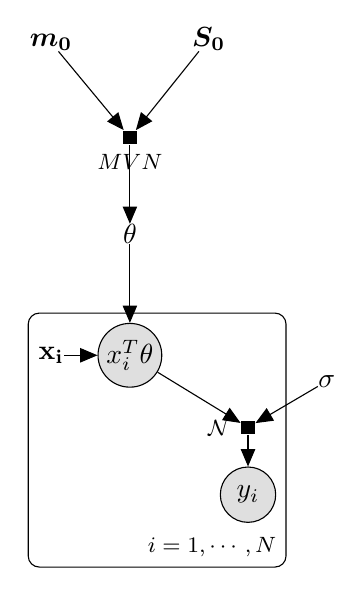
\begin{tikzpicture}   
    \node[obs]                               (xit) {$x_i^T\theta$};
    \node[obs, below=1 of xit, xshift = 1.5cm] (yi) {$y_i$};
    \node[const, xshift=-1cm](xi) {$\mathbf{x_i}$};
    \node[const, above=1 of xit](theta)
    {$\mathbf{\theta}$};
    
    \factor[above=1 of theta] {theta-f} {below:${{MVN}}$} {} {} ; %
    \edge{theta-f}{theta}
    \node[const, above=1 of theta-f, xshift=1cm](sigma) {$\boldsymbol{S_0}$};
    \node[const, above=1 of theta-f, xshift=-1cm](mu) {$\boldsymbol{m_0}$};
    \edge{sigma}{theta-f}
    \edge{mu}{theta-f}

    \factor[above=of yi] {y-f} {left:${\mathcal{N}}$} {} {} ; %
    \node[const, above=1 of yi, xshift=1cm] (sigma) {$\mathbf{\sigma}$};
    \plate{}{(xi)(xit)(yi)}{$i = 1, \cdots, N$};
    \edge{theta}{xit}
    \edge{xit}{y-f}
    \edge{sigma}{y-f}
    \edge{xi}{xit}
    \edge{y-f}{yi}     
\end{tikzpicture}
\end{frame}

\begin{frame}{Bayesian Linear Regression}
In Bayesian linear regression, we consider the model:\\
\begin{equation*} 
\textrm{prior}: \quad p(\boldsymbol{\theta})=\mathcal{N}\left(\boldsymbol{m}_0, \boldsymbol{S}_0\right)
\end{equation*}
\\with $\boldsymbol{m}_0$ and $\boldsymbol{S}_0$ as the mean and covariance matrix and
\begin{equation*}
\textrm{likelihood}: p(y \mid \boldsymbol{x}, \boldsymbol{\theta})=\mathcal{N}\left(y \mid \boldsymbol{\boldsymbol{x}}^{\top} \boldsymbol{\theta}, \sigma^2\right)
\end{equation*}
\end{frame}

\begin{frame}{Bayes Rule}
    % $p(y, \boldsymbol{\theta} \mid \boldsymbol{x})=p(y \mid \boldsymbol{x}, \boldsymbol{\theta}) p(\boldsymbol{\theta})$.

    Given a training set of inputs $\boldsymbol{x}_n \in \mathbb{R}^D$ and corresponding observations $y_n \in \mathbb{R}, n=1, \ldots, N$, we compute the posterior over the parameters using Bayes' theorem as
$$
p(\boldsymbol{\theta} \mid \mathcal{X}, \mathcal{Y})=\frac{p(\mathcal{Y} \mid \mathcal{X}, \boldsymbol{\theta}) p(\boldsymbol{\theta})}{p(\mathcal{Y} \mid \mathcal{X})}
$$
where $\mathcal{X}$ is the set of training inputs and $\mathcal{Y}$ the collection of corresponding training targets. 
\end{frame}

\begin{comment}
\begin{frame}{Bayes Rule}
Now, the denominator $p(\mathcal{Y} \mid \mathcal{X})$ is given as, 
$$
p(\mathcal{Y} \mid \mathcal{X})=\int p(\mathcal{Y} \mid \mathcal{X}, \boldsymbol{\theta}) p(\boldsymbol{\theta}) \mathrm{d} \boldsymbol{\theta}=\mathbb{E}_{\boldsymbol{\theta}}[p(\mathcal{Y} \mid \mathcal{X}, \boldsymbol{\theta})]
$$
The marginal likelihood/evidence, independent of the parameters $\boldsymbol{\theta}$, ensures that the posterior is normalized, i.e., it integrates to 1 . We can think of the marginal likelihood as the likelihood averaged over all possible parameter settings (with respect to the prior distribution $p(\boldsymbol{\theta})$ ).
\end{frame}
\end{comment}
\begin{frame}{Posterior}
We find the closed form solution of posterior $p(\boldsymbol{\theta} \mid \mathcal{X}$ to be a normal distribution with mean $\boldsymbol{m}_N$ and covariance matrix $ \boldsymbol{S}_N$\\
\vspace{10pt}
\begin{equation*}
p(\boldsymbol{\theta} \mid \mathcal{X}, \mathcal{Y})  =\mathcal{N}\left(\boldsymbol{\theta} \mid \boldsymbol{m}_N, \boldsymbol{S}_N\right)
\end{equation*}
\begin{equation*}
 \boldsymbol{S}_N  =\left(\boldsymbol{S}_0^{-1}+\sigma^{-2} \boldsymbol{X}^{\top} \boldsymbol{X}\right)^{-1}
\end{equation*}
\begin{equation*}
\boldsymbol{m}_N  =\boldsymbol{S}_N\left(\boldsymbol{S}_0^{-1} \boldsymbol{m}_0+\sigma^{-2} \boldsymbol{X}^{\top} \boldsymbol{y}\right)
\end{equation*}

where the subscript $N$ indicates the size of the training set.
\end{frame}

\begin{frame} {Proof}
\begin{equation*}
\textrm{Posterior}:  \quad p(\boldsymbol{\theta} \mid \mathcal{X}, \mathcal{Y})=\frac{p(\mathcal{Y} \mid \mathcal{X}, \boldsymbol{\theta}) p(\boldsymbol{\theta})}{p(\mathcal{Y} \mid \mathcal{X})}
\end{equation*}

\begin{equation*}
\textrm{Likelihood}: p(\mathcal{Y} \mid \mathcal{X}, \boldsymbol{\theta})=\mathcal{N}\left(\boldsymbol{y} \mid \boldsymbol{X} \boldsymbol{\theta}, \sigma^2 \boldsymbol{I}\right)
\end{equation*}

\begin{equation*}
\textrm{Prior}: p(\boldsymbol{\theta})=\mathcal{N}\left(\boldsymbol{\theta} \mid \boldsymbol{m}_0, \boldsymbol{S}_0\right)
\end{equation*}

\end{frame}

\begin{frame}{Proof}
The sum of the log-prior and the log-likelihood is
\begin{equation*}
 \log \mathcal{N}\left(\boldsymbol{y} \mid \boldsymbol{X} \boldsymbol{\theta}, \sigma^2 \boldsymbol{I}\right)+\log \mathcal{N}\left(\boldsymbol{\theta} \mid \boldsymbol{m}_0, \boldsymbol{S}_0\right) 
\end{equation*}
\begin{equation*}
=-\frac{1}{2}\left(\sigma^{-2}(\boldsymbol{y}-\boldsymbol{X} \boldsymbol{\theta})^{\top}(\boldsymbol{y}-\boldsymbol{X} \boldsymbol{\theta})+\left(\boldsymbol{\theta}-\boldsymbol{m}_0\right)^{\top} \boldsymbol{S}_0^{-1}\left(\boldsymbol{\theta}-\boldsymbol{m}_0\right)\right)+\text { const }
\end{equation*}
    
\end{frame}

\begin{frame}
We ignore the constant term independent of $\boldsymbol{\theta}$. We now factorize, which yields
\pause $$
\begin{aligned}
& = -\frac{1}{2}\left(\sigma^{-2} \boldsymbol{y}^{\top} \boldsymbol{y}-\textcolor{blue}{2 \sigma^{-2} \boldsymbol{y}^{\top} \boldsymbol{X}\boldsymbol{\theta}}+\textcolor{red}{\boldsymbol{\theta}^{\top} \sigma^{-2} \boldsymbol{X}^{\top} \boldsymbol{X} \boldsymbol{\theta}+\boldsymbol{\theta}^{\top} \boldsymbol{S}_0^{-1} \boldsymbol{\theta}}\right. \\
& \left. \textcolor{blue}{-2\boldsymbol{m}_0^{\top} \boldsymbol{S}_0^{-1} \boldsymbol{\theta}}+\boldsymbol{m}_0^{\top} \boldsymbol{S}_0^{-1} \boldsymbol{m}_0\right) 
\end{aligned}
$$

\pause $$
\begin{aligned}
= & -\frac{1}{2}\left(\textcolor{red}{\boldsymbol{\theta}^{\top}\left(\sigma^{-2} \boldsymbol{X}^{\top} \boldsymbol{X}+\boldsymbol{S}_0^{-1}\right) \boldsymbol{\theta}}-\textcolor{blue}{2\left(\sigma^{-2} \boldsymbol{X}^{\top} \boldsymbol{y}+\boldsymbol{S}_0^{-1} \boldsymbol{m}_0\right)^{\top} \boldsymbol{\theta}}\right)\\
& +\text { const }
\end{aligned}
$$
\end{frame}
\begin{frame}{Posterior}
Now, we evaluate the posterior distribution, 
\begin{equation*}
    p(\boldsymbol{\theta} \mid \mathcal{X}, \mathcal{Y})=\exp (\log p(\boldsymbol{\theta} \mid \mathcal{X}, \mathcal{Y})) \propto \exp (\log p(\mathcal{Y} \mid \mathcal{X}, \boldsymbol{\theta})+\log p(\boldsymbol{\theta}))
\end{equation*}
\begin{equation*}
\propto \exp \left(-\frac{1}{2}\left(\textcolor{red}{\boldsymbol{\theta}^{\top}\left(\sigma^{-2} \boldsymbol{X}^{\top} \boldsymbol{X}+\boldsymbol{S}_0^{-1}\right) \boldsymbol{\theta}}-\textcolor{blue}{2\left(\sigma^{-2} \boldsymbol{X}^{\top} \boldsymbol{y}+\boldsymbol{S}_0^{-1} \boldsymbol{m}_0\right)^{\top} \boldsymbol{\theta}}\right)\right)
\end{equation*}

\end{frame}

\begin{frame}{Normalizing the posterior distribution}
We now normalize this Gaussian distribution into the form that is proportional to $\mathcal{N}\left(\boldsymbol{\theta} \mid \boldsymbol{m}_N, \boldsymbol{S}_N\right)$, i.e., we need to identify the mean $\boldsymbol{m}_N$ and the covariance matrix $\boldsymbol{S}_N$. 

\pause To do this, we use the concept of completing the squares. The desired log posterior is

\pause $$
\begin{gathered}
\log \mathcal{N}\left(\boldsymbol{\theta} \mid \boldsymbol{m}_N, \boldsymbol{S}_N\right)=-\frac{1}{2}\left(\boldsymbol{\theta}-\boldsymbol{m}_N\right)^{\top} \boldsymbol{S}_N^{-1}\left(\boldsymbol{\theta}-\boldsymbol{m}_N\right)+\text { const } \\
=-\frac{1}{2}\left(\textcolor{red}{\boldsymbol{\theta}^{\top} \boldsymbol{S}_N^{-1} \boldsymbol{\theta}}-\textcolor{blue}{2 \boldsymbol{m}_N^{\top} \boldsymbol{S}_N^{-1} \boldsymbol{\theta}}+\boldsymbol{m}_N^{\top} \boldsymbol{S}_N^{-1} \boldsymbol{m}_N\right) .
\end{gathered}
$$
\end{frame}

\begin{frame}{Normalizing the posterior distribution}
We factorize the quadratic form $\left(\boldsymbol{\theta}-\boldsymbol{m}_N\right)^{\top} \boldsymbol{S}_N^{-1}\left(\boldsymbol{\theta}-\boldsymbol{m}_N\right)$ into a term that is quadratic in $\boldsymbol{\theta}$ alone, a term that is linear in $\boldsymbol{\theta}$, and a constant term. This allows us now to find $\boldsymbol{S}_N$ and $\boldsymbol{m}_N$ by matching the expressions, which yields
$$
\begin{aligned}
& \boldsymbol{S}_N^{-1}=\boldsymbol{X}^{\top} \sigma^{-2} \boldsymbol{I} \boldsymbol{X}+\boldsymbol{S}_0^{-1} \\
\Longrightarrow & \boldsymbol{S}_N=\left(\sigma^{-2} \boldsymbol{X}^{\top} \boldsymbol{X}+\boldsymbol{S}_0^{-1}\right)^{-1}
\end{aligned}
$$
and
$$
\begin{aligned}
& \boldsymbol{m}_N^{\top} \boldsymbol{S}_N^{-1}=\left(\sigma^{-2} \boldsymbol{X}^{\top} \boldsymbol{y}+\boldsymbol{S}_0^{-1} \boldsymbol{m}_0\right)^{\top} \\
\Longrightarrow & \boldsymbol{m}_N=\boldsymbol{S}_N\left(\sigma^{-2} \boldsymbol{X}^{\top} \boldsymbol{y}+\boldsymbol{S}_0^{-1} \boldsymbol{m}_0\right) .
\end{aligned}
$$
\end{frame}


\begin{frame}{Posterior Predictive Distribution}
    Goal: Find $p\left(y_* \mid \mathcal{X}, \mathcal{Y}, \boldsymbol{x}_*\right)$

    $$
    \begin{aligned}
        p(y_* \mid \mathcal{X}, \mathcal{Y}, \boldsymbol{x}_*) &= \int p(y_* \mid \boldsymbol{x}_*, \boldsymbol{\theta}) p(\boldsymbol{\theta} \mid \mathcal{X}, \mathcal{Y}) \mathrm{d} \boldsymbol{\theta} \\
        &= \int \mathcal{N}(y_* \mid \boldsymbol{x}_*^\top \boldsymbol{\theta}, \sigma^2) \mathcal{N}(\boldsymbol{\theta} \mid \boldsymbol{m}_N, \boldsymbol{S}_N) \mathrm{d} \boldsymbol{\theta} \\
        &= \mathcal{N}(y_* \mid \boldsymbol{x}_*^\top \boldsymbol{m}_N, \boldsymbol{x}_*^\top \boldsymbol{S}_N \boldsymbol{x}_* + \sigma^2)
        \end{aligned}
        $$

    \pause Two kinds of uncertainty:
    \begin{itemize}
        \item \textbf{Aleatoric uncertainty}: Uncertainty in the data - given as $\sigma^2$
        \item \textbf{Epistemic uncertainty}: Uncertainty in the model - given as $\boldsymbol{x}_*^\top \boldsymbol{S}_N \boldsymbol{x}_*$
    \end{itemize}
\end{frame}

\begin{frame}{Posterior Predictive Distribution}
    \begin{itemize}
        \item TFP blog: Aleatoric v/s Epistemic Uncertainty
        \item MML book: Figure 9.4
    \end{itemize}
\end{frame}

\begin{frame}{Bayesian Updation}
    Bishop book: Figure 3.7
    
\end{frame}

\begin{comment}
\foreach \i in {0,1,2,5,10,20,100}{
  \begin{frame}
    \frametitle{Visualization}
    \includegraphics{blr_\i.png}
  \end{frame}
}
\end{comment}
\end{document}

